\documentclass[tikz,border=14pt]{standalone}
\usepackage[T1]{fontenc}
\usepackage{lmodern}
\usetikzlibrary{positioning,arrows.meta}
\begin{document}
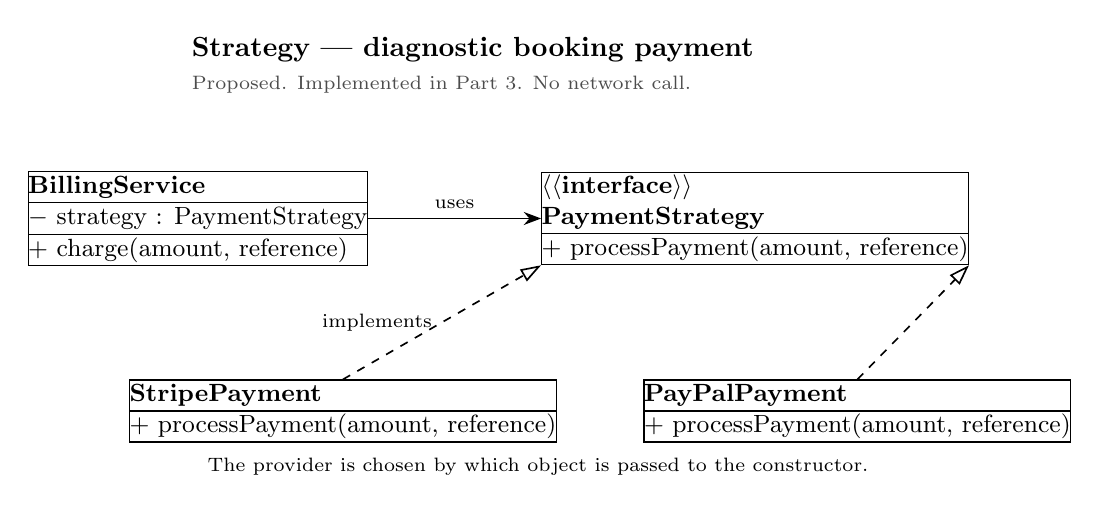
\begin{tikzpicture}[
  font=\small,
  cls/.style={draw, fill=white, inner sep=0pt},
  arr/.style={-{Stealth[length=2.2mm]}, semithick},
  isa/.style={dashed, -{Triangle[open,length=2.6mm]}, semithick}
]
  \node[font=\normalsize\bfseries, anchor=west] at (-0.2,2.15) {Strategy --- diagnostic booking payment};
  \node[font=\scriptsize, anchor=west, text=black!70] at (-0.2,1.7) {Proposed. Implemented in Part 3. No network call.};

  \node[cls] (ctx) {\begin{tabular}{@{}l@{}}
    \textbf{BillingService}\\ \hline
    $-$ strategy : PaymentStrategy\\ \hline
    $+$ charge(amount, reference)
  \end{tabular}};
  \node[cls, right=2.2cm of ctx] (st) {\begin{tabular}{@{}l@{}}
    \textbf{$\langle\langle$interface$\rangle\rangle$}\\
    \textbf{PaymentStrategy}\\ \hline
    $+$ processPayment(amount, reference)
  \end{tabular}};
  \node[cls, below left=1.45cm and -0.2cm of st] (stripe) {\begin{tabular}{@{}l@{}}
    \textbf{StripePayment}\\ \hline
    $+$ processPayment(amount, reference)
  \end{tabular}};
  \node[cls, right=1.1cm of stripe] (paypal) {\begin{tabular}{@{}l@{}}
    \textbf{PayPalPayment}\\ \hline
    $+$ processPayment(amount, reference)
  \end{tabular}};

  \draw[arr] (ctx.east) -- node[above, font=\scriptsize] {uses} (st.west);
  \draw[isa] (stripe.north) -- node[left, font=\scriptsize] {implements} (st.south west);
  \draw[isa] (paypal.north) -- (st.south east);

  \node[font=\scriptsize, anchor=west] at (0,-3.15)
    {The provider is chosen by which object is passed to the constructor.};
\end{tikzpicture}
\end{document}
